\chapter{Articulation Work} % (fold)
\label{cha:articulation_work}

In diesem Kapitel wird das Konzept „Articulation Work“ dargestellt und in den Kontext von menschlicher Arbeit gestellt. Im ersten Teil des Kapitels wird auf die historische Entwicklung des Begriffs „Articulation Work“ und die unterschiedlichen Herangehensweise zu dessen Verständnis eingegangen. Der zweite Teil des Kapitels widmet sich den Aktivitäten, die „Articulation Work“ ausmachen, den Merkmalen, an denen sich gute „Articulation Work“ zeigt, sowie den Möglichkeiten der Unterstützung von „Articulation Work“ durch organisationale und technische Maßnahmen.

\section{Begriffsbestimmung} % (fold)
\label{sec:aw_begriffsbestimmung}

Das Konzept der "Articulation Work" wurde als Erklärungsmodell für eine bestimmte Art von menschlicher Arbeit Mitte der 1980er Jahre von \citet{Strauss85} eingeführt. Neben \citet{Strauss85} tragen auch die Arbeiten von \citet{Gerson86} und \citet{Fujimura87} wesentlich zur Begriffsbestimmung und Konzeptbildung bei. Die vorhandene Literatur, die Bezug auf „Articulation Work“ nimmt, referenziert im Wesentlichen auf diese drei Arbeiten bzw. eine dieser drei Arbeiten. Der Kontext, in dem die Entwicklung der im folgenden vorgestellten Konzepte erfolgte, war die komplexe, von viel Interaktion an zahlreichen Schnittstellen geprägte Arbeit in Krankenhäusern \citep{Strauss85}, in der Wissenschaft \citep{Fujimura87} und in Versicherungsunternehmen \citep{Gerson86}, die die jeweiligen Autoren in mehreren Fallstudien untersuchten. 

Um in der Folge einen einheitlichen Begriffsraum aufspannen zu können, ist vorab der Begriff „Arbeit“ zu klären. Die eben genannten Autoren führen keine explizite Definition an, weshalb hier auf eine Definition zurückgegriffen wird, die im Kontext der folgenden Ausführungen zur „inneren“ Struktur von Arbeit nach „außen“ hinreichend umfassend ist\footnote{Auf eine umfassende Literaturstudie und die Entwicklung eines darauf aufbauenden „Arbeits“-Begriffs wurde hier verzichtet, da dies über den Betrachtungsbereich und Anspruch dieser Arbeit hinausgeht}. \citep{Semmer04} definieren vor dem Hintergrund der Organisationspsychologie „Arbeit“ wie folgt: \emph{„Arbeit ist zielgerichtete menschliche Tätigkeit zum Zwecke der Transformation und Aneignung der Umwelt aufgrund selbst- oder fremddefinierter Aufgaben, mit gesellschaftlicher, materieller oder ideeller Bewertung, zur Realisierung oder Weiterentwicklung individueller oder kollektiver Bedürfnisse, Ansprüche und Kompetenzen.“}. Arbeit ist also ein menschliches Phänomen, Träger von Arbeit sind immer Menschen. Arbeit definiert sich außerdem durch ihre Zielgerichtetheit und findet immer in Interaktion mit der Umwelt statt. Die Ziele, auf die Arbeit ausgerichtet ist, leiten sich aus Aufgaben ab, die sich Menschen selbst setzten können oder die ihnen vorgegeben werden. Diese Aufgaben dienen der Erreichung von individuellen oder kollektiven Bedürfnissen und Ansprüchen bzw. der (Weiter-)Entwicklung von Kompetenzen. Die Bewertung der Zielerreichung muss nicht unbedingt aus materieller Perspektive erfolgen sondern kann auch ideell oder gesellschaftlich begründet sein. In dieser Arbeit wird der Begriff „Arbeit“ vor allem auch im organisationalen Kontext gesehen. Ein wesentlicher Aspekt, der hierbei zu berücksichtigen ist, ist die Arbeitsteilung, also die koordinierte Tätigkeit mehrerer Individuen um ein gemeinsames Ziel zu erreichen (siehe dazu z.B. ). Dies stellt die obige Definition nicht in Frage, erweitert jedoch den Betrachtungsbereich explizit auch auf Arbeit, die gemeinschaftlich durchgeführt wird. 

„Articulation Work“ ist jener Anteil der gesamten durchgeführten Arbeit, der der Abstimmung mit anderen Individuen dient. Diese Abstimmung ist notwendig, um das eigentliche Arbeitsziel erreichen zu können. Arbeit wird von den oben angeführten Autoren als inhärent kooperativer Prozess gesehen, der immer auf Interaktion mit anderen Menschen basiert bzw. diese bedingt (Strauss formuliert diese Annahme in Bezugnahme auf \citet{Hughes71} prägnant mit der Aussage \emph{„work rests ultimately on interaction“}). Diese Annahme erscheint insofern als zulässig, als dass selbst Arbeitsabläufe, die selbst keine Kooperation mit anderen Menschen mit sich bringen, zumindest auf den Ergebnissen anderer Arbeitsabläufe aufbauen oder als Grundlage weiterer Arbeitsabläufe dienen. Interaktion tritt also in jedem Arbeitsprozess zumindest zu Beginn und am Ende in unmittelbarer oder mittelbarer\footnote{Unter "mittelbar" ist hier Interaktion zu verstehen, die nicht im direkten Kontakt zwischen Individuen abläuft sondern lediglich indirekt durch die Ergebnisse eines Arbeitsprozesses (Materialien, Dokumente, \ldots) vermittelt wird.} Form auf.

\textbf{Abbildung, in der kooperative Arbeitsprozesse und solche mit mittelbarer und unmittelbarer Interaktion zu Beginn oder am Ende dargestellt werden}

Jener Teil von Arbeit, der der eigentlichen Zielerreichung dient, wird im hier vorgestellten Erklärungsmodell als „Production Work“ bezeichnet \citep{Fujimura87}. „Production Work“ ist komplementär zu „Articulation Work“ zu sehen und umfasst alle Aktivitäten, die der „Wertschöpfung“ im wörtlichen Sinn dienen. „Production Work“ sind also alle Tätigkeiten, die mit der Schaffung jener Werte (oder Ergebnisse) befasst sind, die durch den Arbeitsablauf erreicht werden sollen.  

\begin{figure}[htbp]
	\centering
		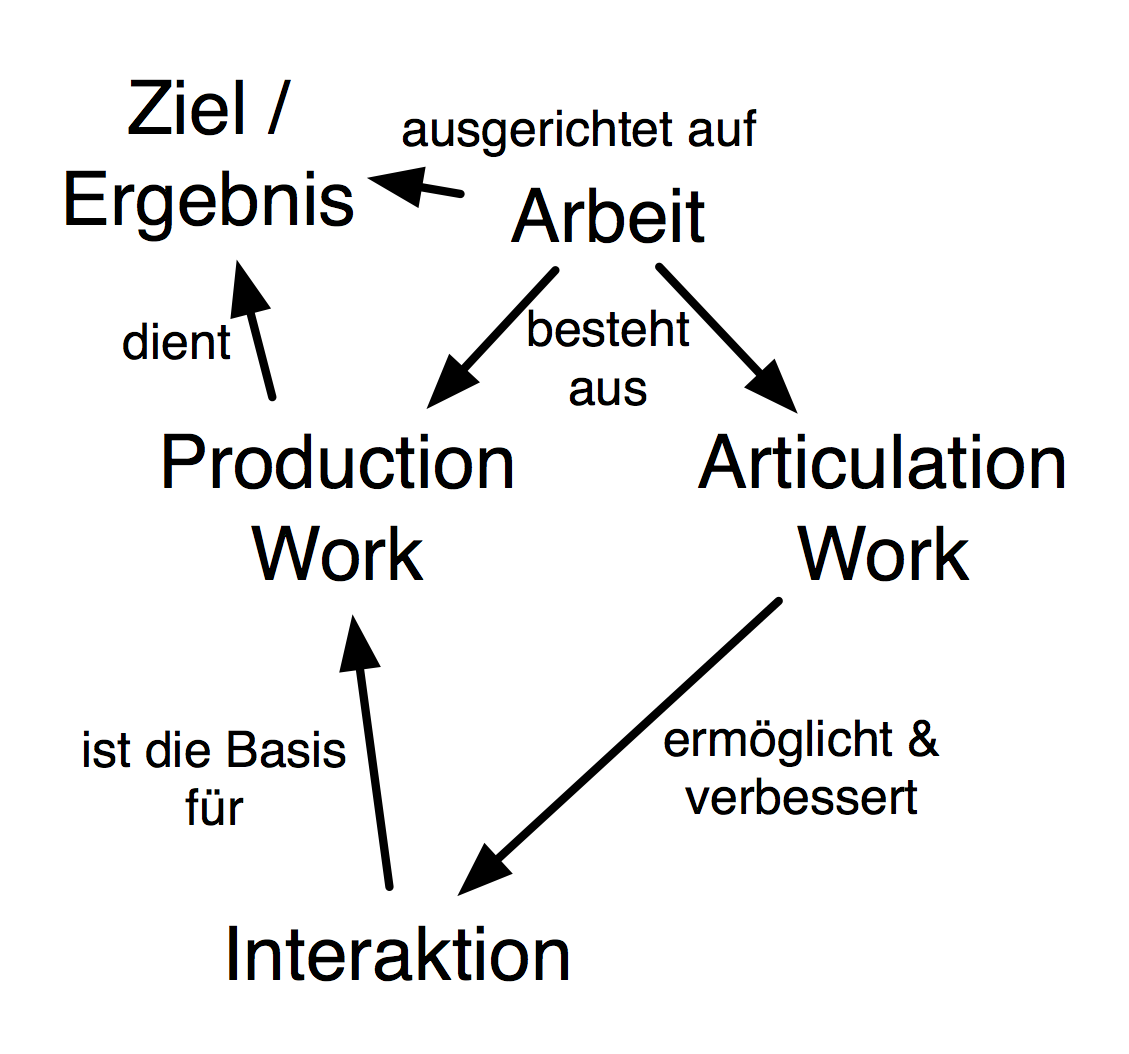
\includegraphics[height=3in]{img/ArticulationWork/ArbeitInteraktion.png}
	\caption{Struktur von Arbeitsabläufen}
	\label{fig:img_ArticulationWork_ArbeitInteraktion}
\end{figure}

Teile eines Arbeitsablaufs dienen also der Zielerreichung an sich („Production Work“). Andere Teile dienen der Abstimmung zwischen den involvierten Akteuren, um ein gemeinsames Verständnis über die jeweiligen Schnittstellen – also die Berührungspunkte zwischen den Tätigkeiten – zu entwickeln (siehe Abbildung \ref{fig:img_ArticulationWork_ArbeitInteraktion}). Diese Entwicklung eines gemeinsamen Verständnisses oder „Koordination“ ist kritisch für den Erfolg von kooperativer Arbeit \citep{Strauss93} und wird als „Articulation Work“ bezeichnet.\footnote{\emph{„Without an understanding of articulation, the gap between requirements and the actual work process in the office will remain inaccessible to analysis. That is, it will be possible to describe tasks in an idealized form but not to describe actual situations.“}\citep{Gerson86}} 

„Articulation Work“ ist also ein Enabler für funktionierende Kommunikation und Zusammenarbeit im eigentlichen Arbeitsablauf. Zentral ist dabei vor allem die gegenseitigen Offenlegung der Annahmen aller beteiligten Personen, die den individuellen Arbeitsbeiträgen zugrunde liegen\footnote{\emph{"Reconciling incommensurate assumptions and procedures in the absence of enforceable standards is the essence of articulation.}\citep[][S. 266]{Gerson86}}. Konkret kann „Articulation Work“ unterschiedliche Ausprägungen annehmen \citep{Gasser86}\citep{Bendifallah87}:
\begin{description}
	\item[Fitting] (bzw. „Accomodation“ \citep{Bendifallah87}) Tätigkeiten zur Planung bzw. Anpassung der Arbeitspraxis an gegebene bzw. veränderte Umweltbedingungen.
	\item[Augmenting] (bzw. „Negotiation of additional [maintainance] activities“ \citep{Bendifallah87}) Planung von zusätzlichen kurz- oder mittelfristigen Tätigkeiten, um das Auftreten von erkannten Problemen zu verhindern. 
	\item[Working around] Entwicklung von Strategien zur Vermeidung des Auftretens von Situationen, in denen Probleme auftreten, ohne deren Ursache zu beseitigen.
\end{description}

 „Articulation Work“ ist keine Tätigkeit, die zu einem bestimmten Zeitpunkt im Arbeitsprozess durchgeführt wird und dann als abgeschlossen betrachtet werden kann. Vielmehr wird „Articulation Work“ immer auch begleitend zur eigentlichen produktiven Arbeit durchgeführt und umfasst neben planenden und koordinierenden Tätigkeiten auch das Erkennen von Fehlentwicklungen bzw. von Situationen, in denen eine erneute  Koordination notwendig ist\footnote{\emph{Articulation consists of all the tasks involved in assembling, scheduling, monitoring, and coordinating all of the steps necessary to complete a production task."}\citep[][S. 266]{Gerson86}}. 

\begin{figure}[htbp]
	\centering
		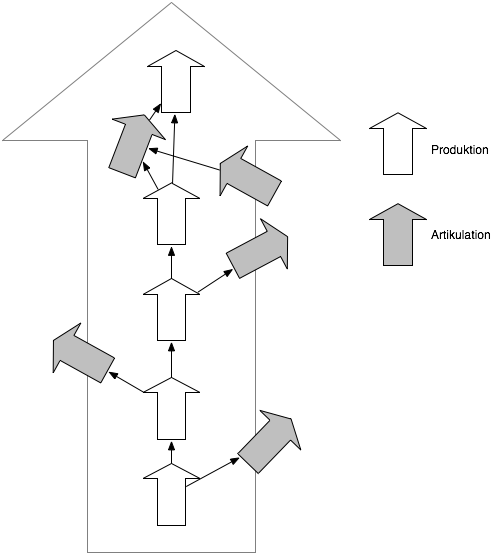
\includegraphics[height=3in]{img/ArticulationWork/ArtikulationProduktion.png}
	\caption{Konzeptualisierung von „Arbeit“ nach \citep{Strauss85} und \citep{Fujimura87}}
	\label{fig:img_ArticulationWork_ArtikulationProduktion}
\end{figure}

Der Begriff „Articulation Work“ ist im Englischen zweideutig und von \citeauthor{Strauss85} auch bewusst so gewählt. Einerseits wird damit ausgedrückt, dass \emph{Arbeit} ("Work") artikuliert wird, andererseits zeigt der Begriff, das die \emph{Artikulation} selbst ebenfalls Arbeit ist (also Zeit und Ressourcen in Anspruch nimmt) und auch also solche wertgeschätzt werden muss \citep{Fujimura87}. „Articulation Work“ ist kein klar abgegrenztes und strukturiertes Konzept – sie tritt je nach Arbeitssituation in unterschiedlichen Spielarten auf. Die Unterscheidung dieser Arten von „Articulation Work“ ist für die Unterstützung derselben relevant und wird daher im folgenden Abschnitt genauer betrachtet.
% section begriffsbestimmung (end)

\section{Ausprägungen von Articulation Work} % (fold)
\label{sec:arten_von_articulation_work}

Wie bereits von \citet{Gerson86} angeführt (siehe oben), argumentiert auch \citeauthor{Strauss88}, dass Artikulation immer passieren muss (und passiert), wo Menschen zusammenarbeiten, um zu vermeiden, dass unbekannte Aspekte Probleme bei der Durchführung der Arbeit verursachen \citep{Strauss88}. „Articulation Work“ ist kein revolutionäres Konzept, sondern fasst Tätigkeiten unter einem Begriff zusammen, die seit jeher Teil jeder Zusammenarbeit zwischen Menschen sind. Grundsätzlich geht Strauss davon aus, dass Artikulation immer abläuft, egal wie einfach oder kompliziert, wie eingespielt oder neuartig eine (Zusammen-)Arbeit ist \citep{Strauss88}. Sehr wohl existieren jedoch Unterschiede in der Qualität der Arbeit, die sich auf die Form der Artikulation auswirken, die zu deren Abstimmung notwendig ist: \emph{„A useful fundamental distinction between classes of interaction is between the routine and the problematic. Problematic interactions involve 'thought', or when more than one interactant is involved then also 'discussion'.“} \citep{Strauss93}. Dieses Zitat zeigt im Übrigen auch, dass „Interaction“ im Sinne von Strauss nicht unbedingt ein kollektives Phänomen ist, sondern auch individuell (im Bezug auf die (unbelebte) Umgebung) auftreten kann.

Je komplexer („problematic“) eine Interaktion ist, desto notwendiger wird laut Strauss eine explizite Beschäftigung mit dem Vorgang der Artikulation. Bei einfachen, eingespielten („routine“) Interaktionen bleibt die Artikulation zumeist implizit, verborgen und informell \citep{Hampson05} (entsprechend der „Sozialisation“ im aus der Domäne der Wissensgenerierung und -teilung stammenden SECI-Zyklus \citep{Nonaka95}). Ein grundlegendes Problem, dass Artikulation für jeden noch so einfach erscheinend Arbeitsvorgang potentiell relevant macht, spricht Strauss mit den Worten von Hughes unmittelbar nach der Definition von „problematic interaction“ an: \emph{„[O]ne man's routine of work is made up of the emergencies of other people“} \citep{Hughes71} zitiert nach \citep{Strauss93}.

„Articulation Work“ tritt also in zwei Qualitäten auf. Ist der Bedarf zur Abstimmung bekannt und werden Tätigkeiten zur Abdeckung dieses Bedarf bewusst durchgeführt, so spricht man von \emph{expliziter} „Articulation Work“ \citep{Strauss88} \citep{Fjuk97}. Die Abstimmung von Tätigkeiten, die ständig während der Zusammenarbeit unbewusst ausgeführt wird, bezeichnet man als \emph{implizite} „Articulation Work“\footnote{\emph{The explicit articulation is thus connected to the planning and decisions regarding the salient dimensions of work -- who, what, when, how -- while implicit articulation is invaluable when carrying out activities in situated circumstances, in order to handle contingencies.}\citep[][S.5]{Fjuk97}}. Letztgenannte Art ist es auch, die von den Arbeitenden „automatisch“ zur Anwendung gebracht wird, sobald Änderungen in der Arbeitsumgebung oder Probleme auftreten \citep{Strauss88}. Implizite „Articulation Work“ stößt aber an ihre Grenzen, wenn die Arbeitssituation als „problematisch“ \citep{Strauss88} oder „komplex“ \citep[][S. 23f]{Schmidt90} wahrgenommen wird. Es wird dann notwendig, dezidierte Abstimmungs-Aktivitäten anzustoßen, also explizite „Articulation Work“ durchzuführen.

Neben der Unterscheidung zwischen impliziter und expliziter Articulation Work anhand der Komplexität der zugrunde liegenden Interaktion führt Strauss keine systematische Betrachtung von Articulation Work hinsichtlich deren Ausprägungen durch. Offensichtlich wird in seinen Texten jedoch, dass es Articulation Work als beobachtbares und eindeutig also solche identifizierbares Phänomen nicht gibt. Abhängig vom betrachteten Arbeitsablauf, der Arbeitsumgebung und den beteiligten Personen zeigt sich Articulation Work in unterschiedlichen Formen.

In der Literatur existieren zwei Ansätze zur Differenzierung zwischen unterschiedlichen Arten von Articulation Work. \citet{Fjuk97} stellen Articulation Work der Activity Theory \citep{Leontev78} gegenüber und unterscheiden so verschiedene Ebenen. \citet{Hampson05} führen ein Raster ein, das Articulation Work hinsichtlich der Art des Arbeitsprozesses unterschiedet, in dem sie zur Anwendung kommt. Beide Ansätze werden in der Folge im Detail beschrieben und bezüglich ihrer Implikationen für diese Arbeit betrachtet.

\subsection{Unterscheidung nach Fjuk, Smørdal und Nurminen}
\label{sub:arten_fjuk}

\citet{Fjuk97} betrachten Articulation Work im Kontext von \gls{CSCW} und versuchen ein konzeptionelles Framework zu entwickeln, das die Rolle von Computersystemen im Kontext indvidueller und kollektiver Tätigkeiten erklärt -- sie entwickeln also ein Erklärungsmodell für die Funktionsweise sozio-technischer Systeme \citep{Emery60}. Während die Implikationen von „Articulation Work“ für \gls{CSCW} an dieser Stelle nicht näher von Belang sind ist aber das theoretische Framework, das die Autoren ihren Ausführungen zu Grunde legen von Interesse. 

\citet{Fjuk97} beziehen sich bei ihren Überlegungen auf die „Activity Theorie“ (Tätigkeits-Theorie), die maßgeblich von \citep{Leontev72} geprägt wurde. Die Autoren argumentieren, dass diese einen Ansatzpunkt bietet, die von Strauss als relevant erkannten aber nicht näher behandelten „externen Faktoren“, die Arbeit beeinflussen, zu berücksichtigen. Der Begriff der „externen Faktoren“ wird mit allen Einflussfaktoren beschrieben, die nicht unmittelbar Teil des Arbeitsablaufs sind sondern technologischer, organisationaler, kultureller, wirtschaftlicher oder physiologischer Natur sind. 

Ohne an dieser Stelle näher auf die „Activity Theory“ \footnote{für eine allgemein verständliche Einführung unter Berücksichtigung der praktischen Implikationen siehe \citet{Dahme97} oder \citet{Nardi06}} einzugehen, seien hier die drei Kernkonzepte der Theorie erwähnt:
\begin{itemize}
	\item Activity (Tätigkeit)
	\item Action (Aktion)
	\item Operation (Operation)
\end{itemize}

Diese drei Konzepte bilden eine Hierarchie, in denen eine „Activity“ an oberster Stelle steht. Eine „Activity“ ist eine menschliche Tätigkeit, die durch ein Motiv getrieben ist und der (vorerst) individuellen Bedürfnisbefriedigung dient. Eine „Activity“ setzt sich aus mehreren „Actions“ zusammen, die jede für sich ein aus dem Motiv heraus begründbares Ziel haben und zur Bedürfnisbefriedigung direkt oder indirekt betragen. „Actions“ setzen sich wiederum aus „Operations“ zusammen, also einzelnen, nicht mehr bewusst ausgeführten Handlungen, die durch die Bedingungen des jeweiligen Umgebungskontexts bestimmt werden. Während sie lernen, transformieren Individuen laufend „Actions“ zu „Operations“, automatisieren also deren Ausführung, sodass sich die kognitive Belastung verringert (als klassisches Beispiel kann hier das Erlernen des Autofahrens dienen).

Die „Activity Theory“ beschreibt als psychologisches Modell vorerst das Individuum und dessen Verhalten. In sozialen Systemen, die auf Interaktion basieren, stößt das Modell jedoch an die Grenzen der erklärbaren Phänomene. \citet{Engestrom87} baut auf der klassischen „Activity Theory“ auf und erweitert diese um den Aspekt der Gemeinschaft sowie der Interaktion in dieser bzw. der Rolle von Artefakten („Objects“) in derartigen Settings. \citet{Fjuk97} bemängeln aber in ihren Ausführungen, dass \citeauthor{Engestrom87} in seinen Ausführungen abstrakt bleibt und nicht den Konkretisierungsgrad der originären „Activity Theory“ erreicht, was das Zusammenspiel der unterschiedlichen Ebenen („Activity“, „Action“ und „Operation“) betrifft.

Hinsichtlich der näheren Betrachtung von Articulation Work unterscheiden \citet{Fjuk97} in Bezugnahme auf \citet{Strauss93} vorerst zwei Ebenen („levels“) von „Articulation Work“, namentlich „planned“ und „situated Articulation Work“. Diese Unterscheidung korrespondiert den Autoren nach im Wesentlichen mit der Unterscheidung zwischen „expliziter“ und „impliziter Articulation Work“, da erstere geplant und zu einem zuvor bestimmten Zeitpunkt ausgeführt wird und zweitere ad-hoc, bei Bedarf, und eher informell abläuft. Diese Entsprechung steht jedoch teilweise im Konflikt mit späteren Aussagen in der Arbeit, in der auf „situated Articulation Work“ Bezug genommen wird, die aber ob der herausfordernden Natur des Arbeitsablaufs „expliziter“ abzulaufen habe \citep[][S. 15]{Fjuk97}

Unter Einbeziehung der „Activity Theory“ und basierend auf der Unterscheidung zwischen „Activity“, „Action“ und „Operation“ führen \citet{Fjuk97} außerdem zwei unterschiedliche Arten von „Articulation Work“ ein, die sich in ihren Bezugspunkten unterschieden und jeweils für den Fall individueller und kollektiver Tätigkeiten bzw. Aktionen betrachtet werden.  

\begin{description}
	\item[Articulation of action within individual activity] Die Artikulation von Aktionen innerhalb einer Tätigkeit entspricht einer bewussten Planung eines Vorgehens zur Erreichung von definierten Zielen. Diese Form von „Articulation Work“ ist per Definition geplant („planned“) und damit explizit. Sie umfasst lediglich Planungsaktivitäten eines Individuums und umfasst die Klärung der Fragen „wer“ (in diesem Zusammenhang das Individuum selbst oder andere) „was“ (im Sinne des zu erreichenden Ziels) „wo“ (im Sinne des örtlichen, zeitlichen oder organisationalen Kontexts) „wie“ (im Sinne der Operationalisierung der Aktionen zur Zielerreichung) arbeitet.
	\item[Articulation of operation within action in individual activities] Die Auswahl und Ausführung von Operationen im Kontext einer Aktion erfolgt zumeist nicht bewusst basierend auf Erfahrungswissen. Tatsächlich kann die Auswahl von adäquaten Operationen als ein permanenter Fluss von mit der produktiven Arbeit verwobenen („situated“) „Articulation Work“-Vorgängen gesehen werden, der implizit auch in individuellen Arbeitssituationen abläuft. In diesem Zusammenhang ist es wichtig zu erwähnen, dass Operationen in „problematischen“ Situationen (im Sinne von Strauss) zu Aktionen werden können, die nicht mehr unbewusst und automatisiert ablaufen können. Mit dieser Transformation wird auch die „Articulation Work“ explizit und muss dass individuelle Vorgehen der geänderten Situation anpassen. 
	\item[Articulation of individual action within collective activity] Die Artikulation von Aktionen innerhalb eine kollektiven Tätigkeit geht in den Gegenständen der Artikulation über die im individuellen Fall zu berücksichtigenden Planungsaspekte („wer“, „was“, „wo“, „wie“) hinaus. Zusätzlich müssen um Zuge der Artikulation die Regeln der Kommunikation und Arbeitsteilung zwischen den am Arbeitsprozess Beteiligten artikuliert werden. Die Artikulation umfasst hier auch die die gegenseitige Offenlegung und Kenntnisnahme der individuellen „kognitiven Strukturen“ und existierender Annahmen über den Arbeitsablauf.
	\item[Articulation of individual operation within action in collective activity] Im Gegensatz zur individuellen Artikulation von Operationen im Kontext von Aktionen ist diese im kollektiven Fall seltener implizit abzuwickeln. Unterschiedliche Auffassungen über Herangehensweisen oder Missverständnisse bedürfen zum Teil einer expliziten Klärung  um die Zielerreichung zu gewährleisten. Operationen werden hier damit oft auf die Ebene von Aktionen gehoben und bewusst ausgehandelt.
	\item[Articulation of collective action in collective activity] Die Kategorie der kollektiven Aktion wird von \citep{Fjuk97} nicht im Detail behandelt, da die „Activity Theory“ selbst diese nicht behandelt und auch keinerlei anderen diesbezüglich verwendbaren Forschungsergebnisse verwendbar wären. Jede Tätigkeit involviert auch kollektive Aktionen wie Aushandlungen, Konsensfindung oder gemeinsame Problemlösung. Bei der Artikulation von kollektiven Aktionen müssen alle beteiligten Individuen ihre Perspektive, ihr Wissen und ihre Überlegungen einbringen um die gemeinschaftliche Entwicklung voranzutreiben. \citet{Fjuk97} treffen hier keine Aussagen hinsichtlich der Implikationen für „Articulation Work“.
	\item[Articulation of operations within collective actions in collective activity] Bei Zusammenarbeit auf Aktionsebene kann es durch die per Definition nicht bewusst geplante Durchführung der individuellen Operationen zu Zielerreichung der kollektiven Aktion zu konfliktionären Situationen kommen. Vor allem, wenn die individuellen Vorstellungen des Arbeitsablaufs divergieren („weak common conceptual structures“), kann es notwendig sein, explizite „Articulation Work“ anzustoßen, um diese Vorstellungen offenzulegen und abzugleichen.
\end{description}

Innerhalb eines Arbeitsablaufs können auch mehrere der hier beschriebenen Kategorien auftreten. Teile von Arbeitsabläufen können durch Änderungen im Arbeitskontext die Kategorie wechseln und somit mehr oder weniger explizite „Articulation Work“ notwendig machen. Durch die Unterscheidung zwischen kollektiver Tätigkeit und Aktion wird es möglich „Articulation Work“ je nach Enge der Interaktion und den damit auftretenden unterschiedlichen Artikulationsbedürfnissen entsprechend auszulegen.

\subsection{Unterscheidung nach Hampson und Junor}
\label{sub:arten_hampson}

\citep{Hampson05} verwenden „Articulation Work“ als Framework zur Erklärung von „interactive customer service“, also dem jenen Kundenbeziehungen, bei denen die Interaktion zwischen Anbieter und Kunden im Vordergrund steht. Im Rahmen dieser Arbeit zeigen die Autoren auch die historische Entwicklung des Begriffs „Articulation Work“ auf und entwickeln einen Raster zur Einordnung unterschiedlicher Ausprägungen von Arbeit, die wiederum unterschiedliche Arten von „Articulation Work“ bedingen. Dieses Raster ist hier von Interesse.

Bezugnehmend auf \citep{Strauss93} unterschieden die Autoren einerseits zwischen Arbeitsabläufen, die \emph{routine} sind, und solchen, die \emph{non-routine} sind. Außerdem kann zwischen Arbeitsabläufen unterschieden werden, die \emph{visible} oder \emph{invisible} sind \citep{Star99}. Während \emph{visible work} all jene Arbeitsabläufe umfasst, die als solche wahrgenommen werden, bezieht sich \emph{invisible work} auf alle Arbeitsabläufe, die stattfinden aber nicht „offiziell“ wahrgenommen werden (also etwa nicht in einem Prozessmodell aufscheinen).  Daraus ergeben sich vier zu unterscheidende Settings, in denen „Articulation Work“ stattfindet und die sich sowohl in der konkret als „Articulation Work“ ausgeführten Tätigkeit als auch in der möglichen methodischen und/oder technischen Unterstützung unterscheiden.

\begin{description}
	\item[Visible routine work] beschreibt jene Arbeitsabläufe, die von klassischen Management-Ansätzen erfasst werden, formalisiert werden können und in Unternehmen oft normiert vorgegeben sind (etwa in Form von Prozessmodellen oder durch die Vorgaben eines Workflow-Management-Systems). „Articulation Work“ findet hier zu definierten Zeitpunkten und explizit ausgelöst statt, um die normierten Abläufe zu definieren bzw. diese an veränderte Rahmenbedingungen anzupassen. 
	\item[Visible non-routine work] beschreibt Arbeitsabläufe in Umgebungen, die so dynamisch sind, dass normierte Abläufe aufgrund der raschen, nicht absehbaren Veränderungen der Anforderungen nicht sinnvoll einsetzbar sind. „Articulation Work“ tritt hier regelmäßig implizit und explizit auf, da jede Veränderung eine -- je nach Ausmaß der Veränderung implizite oder explizite -- Neuabstimmung der Zusammenarbeit nach innen und außen benötigt.
	\item[Invisible routine work] umfasst all jene Arbeitsabläufe in Unternehmen, die zwar etabliert sind, von den traditionellen Steuer- und Kontroll-Werkzeugen im Unternehmen jedoch nicht erfasst werden. Sie sind formal nicht normiert, treten jedoch so regelmäßig auf, das sich eine routinemäßige Herangehensweise herausbildet. Articulation Work läuft hier bei Veränderungen der Rahmenbedingungen zumeist implizit ab und sorgt dafür, dass die Interaktion zwischen den Beteiligten weiter funktioniert. Explizite „Articulation Work“ unter Einbeziehung der betroffenen Personen kann hier dafür sorgen, Arbeitsabläufe dieser Kategorie in den Bereich der „visible routine work“ überzuführen.
	\item[Invisible non-routine work] umfasst jene Arbeitsabläufe, die zur Behandlung von unvorhergesehenen Anforderungen durchgeführt werden und die nach außen hin nicht sichtbar wird. Typisch treten derartige Situationen bei Ausnahmefällen in etablierten Arbeitsabläufen auf, bei denen die Tätigkeiten zu Wiederherstellung einer „regelkonformen“ Situation oft nicht durch Steuer- und Kontrollelemente erfasst werden und durch die Einzigartigkeit der Ausnahme oder des Kontexts, in dem diese auftritt, keine etablierten Handlungsmuster existieren. „Articulation Work“ ist hier ad-hoc notwendig, um adäquat auf die Anforderungen der Umwelt reagieren zu können. Sowohl explizite und implizite „Articulation Work“ kann hier zu Anwendung kommen, wobei als Entscheidungskriterien zwischen diesen beiden Ausprägungen die wahrgenommene Komplexität der Situation sowie die zur Lösung zur Verfügung stehende Zeit zu berücksichtigen sind.
\end{description}

In unterschiedlichen Arbeitssituationen können diese vier Kategorien auch kombiniert auftreten. Auch hier können manche Arbeitsabläufe durch erfolgreich durchgeführte „Articulation Work“ in eine andere Kategorie verschoben werden, wo der Bedarf an laufender ad-hoc Abstimmung geringer oder nicht vorhanden ist. Andere Arbeitsabläufe sind ihrer Natur nach nicht strukturierbar und formalisierbar, so dass „Articulation Work“ ein inhärenter Bestandteil des Ablaufs ist und trotz wiederholter Durchführung auch bleibt.

\subsection{Zusammenfassung} % (fold)
\label{sub:aw_zusammenfassung}

In diesem Abschnitt wurden drei Arbeiten näher vorgestellt, die sich der  Strukturierung des Konzepts „Articulation Work“ widmen. Die grundlegende Strukturierung bietet bereits \citet{Strauss85} (bzw. \citet{Strauss88} und \citet{Strauss93}). Die beiden übrigen Arbeiten bauen auf \citeauthor{Strauss85} auf und vertiefen das Verständnis von „Articulation Work“ weiter, in dem sie vor allem den im Zuge von „Articulation Work“ behandelten Gegenstand weiter ausdefinieren und strukturieren. Die beiden Arbeiten gehen hierbei unterschiedliche Wege. \citet{Fjuk97} setzen „Articulation Work“ in Beziehung zur aus der Psychologie stammenden „Activity Theory“ während \citet{Hampson05} im Kontext der Soziologie bleibt und neben den Arbeiten von Strauss z.B. auch auf \citep{Star99} aufbaut.

Fasst man die Konzepte zur Strukturierung von „Articulation Work“ aus allen drei Arbeiten zusammen, so ergib sich folgender Überblick: 

\begin{itemize}
	\item Art der „Articulation Work“
	\begin{itemize}
		\item implizit vs. explizit
		\item situated vs. planned
	\end{itemize}
	\item Gegenstand der „Articulation Work“
	\begin{itemize}
		\item routine vs. non-routine work bzw.
		\item routine vs. problematic interaction (mit der belebten oder unbelebten Umwelt)
		\item visible vs. invisible work
		\item individual activity vs. collective activity vs. collective action
	\end{itemize}
	\item Abstraktionsgrad des Gegenstandes der „Articulation Work“
	\begin{itemize}
		\item activity-action vs. action-operation
	\end{itemize}
\end{itemize}

Bezüglich der unterschiedlichen Arten von „Articulation Work“ sind zwei Gegensatzpaare zu identifizieren, die orthogonal zueinander stehen (auch wenn die Hauptachse „implizit -- situated“ vs. „explizit -- planned“ ist). „Situated Articulation Work“ tritt ungeplant während des Arbeitsablaufs auf und dient der ad-hoc- Abstimmung. Obwohl diese in den meisten Fällen implizit abläuft, sind doch Fälle vorstellbar, in denen eine explizite, d.h. bewusst durchgeführte, „Articulation Work“ sinnvoll bzw. notwendig ist (siehe weiter unten -- Gegenstand der „Articulation Work“). „Planned Articulation Work“ hingegen ist immer explizit, die Kombination von geplanter und implizit, d.h. unbewusst durchgeführter, „Articulation Work“ ist nicht sinnvoll.

Hinsichtlich des Gegenstandes von „Ariculation Work“ sind vier unterschiedliche Unterscheidungskategorien zu identifizieren, die wiederum zum Teil orthogonal sind. Die Ausprägungen der jeweiligen Kategorien weisen zum Teil auf die Art der durchzuführenden Articulation Work hin. 

Die Kategorie „routine -- non-routine work“ bezieht sich darauf, ob der fragliche Arbeitsablauf für die beteiligten Personen alltäglich ist und unter bekannten Rahmenbedingungen stattfindet oder nicht. Je stärker der „non-routine“-Anteil in einem Arbeitsablauf zum Tragen kommt, desto expliziter muss im Allgemeinen die „Articulation Work“ sein -- bei Routine-Arbeit ist der Bedarf an Articulation gering und beschränkt sich auf implizit durchführbare Detailabstimmungen zwischen den Beteiligten. 

Obwohl vordergründig unterschiedlich bezieht sich die nächste Kategorie „routine -- problematic interaction“ auf den gleichen Sachverhalt. \citet{Strauss93}, von dem diese Unterscheidung stammt, bezeichnet Interaktion als die Grundlage von Arbeitsabläufen und als wesentlichen Bestandteil derselben. Der „routine“-Begriff kann deshalb mit jenem der zuvor beschriebenen Unterscheidung geleichgesetzt werden. Der Begriff der „problematic interaction“ beschreibt insofern das gleiche Phänomen wie der der „non-routine work“ als dass er sich ebenfalls auf die erhöhte kognitive Belastung der beteiligten Personen bei der Zielerreichung bezieht. Dementsprechend impliziert „problematic interaction“ eine explizite „Articulation Work“, während „routine interaction“ durch implizite „Articulation Work“ produktiv gehalten werden kann.

Die Unterscheidung zwischen „visible“ und „invisible work“ bezieht sich auf die Kenntnisnahme eines Arbeitsablaufs in seinem Durchführungskontext und dessen durch andere, vor allem auch übergeordnete Instanzen. Während „visible work“ definierten Aufgaben dient, formalisiert werden kann und durch Steuer- und Kontrollinstrumente oder organisationale Unterstützungswerkzeuge erfasst werden kann, bleibt „invisible work“ im organisationalen Kontext verborgen und ist nur für die handelnden Individuen sichtbar (und wird dementsprechend auch organisational nicht unterstützt und wertgeschätzt). Für „Articulation Work“ hat dies per se keine unmittelbaren Auswirkungen, außer dass „visible work“ immer ein Ergebnis expliziter „Articulation Work“ ist. Dies bedeutet gleichzeitig, dass explizite „Articulation Work“ (unter Einbeziehung sowohl der unmittelbar am Arbeitsablauf beteiligten Personen als auch der „übergeordneten“ Instanzen) dazu beitragen kann, „invisible work“ zu „visible work“ zu machen (siehe dazu auch \citep{Fujimura87}). „Articulation Work“ ist somit ein Mittel, einen Abgleich zwischen dem offiziellen (organisational festgeschriebenen) Verständnis eines Arbeitsablaufs und dem tatsächlichen Ablauf, wie er in der Praxis ausgeführt wird, durchzuführen. „Articulation Work“ kann damit eine Realisierung eines organisationalen Lernschritts sein, der im Sinne von \citet{Argyris78} die „espoused theories“ (die offiziell veröffentlichten Theorien über Arbeit) mit den „theories-in-use“ (die tatsächlich handlungsleitenden Theorien) abgleicht bzw. im Sinne von \citet{Sachs95} einen „tacit organisational view“ in einen „explicit organisational view“ überführen (siehe dazu auch die Ausführungen in Kapitel XY (Einführung)).

Die Enge der notwendigen Kooperation bei der Durchführung eines Arbeitsablaufs (festgemacht an den Handlungs-Kategorien der „Activity Theorie“) ist Gegenstand der letzten Kategorie. „Individual activity“ beschreibt Arbeitsabläufe, die im Wesentlichen von einem Individuum ausgeführt werden und lediglich an den Schnittstellen zu Beginn und am Ende Interaktion benötigen. „Collective Activity“ beschreibt Arbeitsabläufe, in denen mehrere Individuen klar abgegrenzte Teile der Arbeit übernehmen und Interaktion an festgelegten Schnittstellen bzw. zu festgelegten Zeitpunkten stattfindet. Dies entspricht im Wesentlichen der klassischen Arbeitsteilung in Unternehmen. „Collective Action“ beschreibt tatsächlich kollaborative Arbeit im engeren Sinn, deren Durchführung nur durch enge Interaktion mehrere Individuen auch in Detailaspekten notwendig ist. Je enger die Kooperation, desto notwendiger wird „Articulation Work“, wobei diese in allen Fällen sowohl in ihrer impliziten als auch expliziten Ausprägung zum Einsatz kommen kann. 

Zur Identifikation der im Einzelfall sinnvollen Variante von „Articulation Work“ (implizit oder explizit) ist die Berücksichtigung der letztgenannten Unterscheidung hinsichtlich des Abstraktionsgrades der „Articulation Work“ notwendig. Beschäftigt sich „Articulation Work“ mit der abstrakteren Ebene zwischen „activity“ und „action“, steht vorrangig die Betrachtungsdimension „Was?“ (also die Ziele und das generelle Vorgehen) im Zentrum. Bei Arbeitsabläufen, die „non-routine“ sind, kommt dabei sowohl „situated“ als auch „planned“ eher explizite Articulation Work zum Einsatz. Bei „routine“-Arbeitsabläufen ist Articulation Work auf dieser Ebene „situated“ nicht notwendig und kommt nur zu Anwendung, wenn der Ablauf selbst („planned“) hinterfragt werden soll (und ist dann seiner Natur nach explizit). Auf der konkreten Ebene zwischen „action“ und „operation“ (also der Frage nach dem „Wie?“) kommt in individuell abgehandelten Arbeitsabläufen vorrangig implizite „Articulation Work“ zum Einsatz. Treten unvorhergesehene Probleme auf oder erscheinen etablierte Operationen nicht mehr adäquat, kommt zur Klärung wieder explizite Articulation Work zum Einsatz. In kollektiven Arbeitsprozessen ist die Enge der Interaktion entscheidend. Bei klar separierbaren Arbeitsanteilen (also bei Interaktion auf „activtiy“-Ebene) bleibt die Entscheidung zur konkreten Umsetzung beim Individuum und die „Articulation Work“ im Normalfall implizit (Ausnahmen siehe Ausführungen zur individuellen Arbeitsabläufen). Bei Arbeitsabläufen mit enger Interaktion auf Aktionsebene muss diese im Normalfall „planned“ im Vorhinein durch explizite „Articulation Work“ ausgehandelt werden. Während des Arbeitsablaufs (also „situated“) kann wiederum implizite „Articulation Work“ zurückgegriffen werden, wobei auf Grund der Anzahl der beteiligten Personen die Wahrscheinlichkeit steigt, das ein beteiligtes Individuum die Interaktion als „problematic“ empfindet und dies wiederum explizite „Articulation Work“ notwendig macht.

Insgesamt können drei Arten von „Articulation Work“ unterschieden werden:
\begin{itemize}
	\item „situated“ implizite „Articulation Work“
	\item „situated“ explizite „Articulation Work“
	\item „planned“ explizite „Articulation Work“
\end{itemize}
Die Kombination „planned“ - implizit ist insofern nicht sinnvoll, als dass geplante „Articulation Work“ deren bewusste Durchführung impliziert und diese deshalb immer explizit ist.

Der am häufigsten auftretende Fall von „Articulation Work“ ist jener, der „situated“ (also im Zuge des Arbeitsprozesses) implizit (also unbewusst) auftritt. Implizite „Articulation Work“ ist integraler Bestandteil jedes Arbeitsprozesses. Explizite „Articulation Work“ ist bei „situated“ Durchführung als Eskalationsstufe zu sehen. Wenn der Arbeitsprozess von zumindest einem Beteiligten als problematisch („problematic“ bzw. „non-routine“) angesehen wird, ist eine bewusste Beschäftigung mit der Arbeitsausführung auf abstrakter („Was?“) und / oder konkreter („Wie?“) Ebene notwendig. Sobald die Probleme beseitigt sind, ist eine Fortsetzung der Arbeit mit impliziter „Articulation Work“ möglich. Geplante Articulation Work dient der initialen Planung und Abstimmung 
von neuen Arbeitsabläufen bzw. der Reflexion und Verbesserung von bereits existierenden Arbeitsabläufen. Sie beschäftigt sich eher mit abstrakten Aspekten des Arbeitsablaufs („Was?“), nur im Falle von enger Kooperationsnotwendigkeit in konkreten Tätigkeiten kann auch die Frage nach dem „Wie?“ relevant sein. Geplante explizite „Articulation Work“ ist auch das Mittel der Wahl „invisible work“ auf organisationaler Ebene sichtbar zu machen und damit Wissen über die tatsächliche Durchführung von Arbeitsabläufen in einer Organisation zu verteilen bzw. deren formale Anerkennung zu ermöglichen.

% subsection aw_zusammenfassung (end)
% section arten_von_articulation_work (end)

\section{Unterstützung von Articulation Work} % (fold)
\label{sec:unterstützung_von_articulation_work}

Nach den ersten Arbeiten von Strauss zum Thema „Articulation Work“ wurde das Konzept rasch als Erklärungsmodell für die Vorgänge im Zuge kooperativer Arbeit aufgenommen. Bereits \citeyear{Gerson86} verweisen \citeauthor{Gerson86} auf die Notwendigkeit einer expliziten Unterstützung von „Articulation Work“\footnote{\emph{„Methods for analyzing 
due process means, in this perspective, explicit procedures for evaluating and reconciling incompatibilities among different bodies of tacit local knowledge.“}\citep[][S. 266]{Gerson86}}. Anhand der historischen Entwicklung von Mitte der 1980er-Jahre bis Ende des ersten Jahrzehntes des neuen Jahrtausends werden im Folgenden Maßnahmen zur Unterstützung beschrieben und in den jeweiligen Anwendungskontext gesetzt. Hierbei werden alle Arbeiten berücksichtigt, die sich direkt auf den von Strauss geprägten „Articulation Work“-Begriff beziehen. In der Literatursuche wurden dazu Datenbanken aus den Bereichen Informatik, Psychologie, Soziologie, den Wirtschaftswissenschaften sowie der Organisationslehre durchsucht. Nach der initialen Suche wurde jeweils auch die in den gefundenen Arbeiten referenzierte Sekundärliteratur aufgearbeitet. Des weiteren wurden mit Hilfe von rückwärts verlinkenden Datenbanken (wo vorhanden) Publikationen erfasst, die die bislang gefundenen Arbeiten referenzieren und diese hinsichtlich ihrer Relevanz überprüft. Insgesamt ergab sich so eine Sammlung von 47 Publikationen (inklusive der hier nicht nochmals behandelten grundlegenden Arbeiten, die bereits oben beschrieben wurden). Von diesen 47 Publikationen trafen XY eine Aussage zu Aspekten, die auf die Unterstützung von „Articulation Work“ abzielen. Die übrigen Arbeiten verwenden „Articulation Work“ als Erklärungs-Framework für Fallstudien und werden weiter unten zusammenfassend angeführt ohne näher auf sie einzugehen.

Zur strukturierten Umsetzung der Betrachtung der Unterstützung von „Articulation Work“ wird ein einheitlicher Raster angewandt, anhand dessen die aus unterschiedlichen Forschungsgebieten stammenden und in unterschiedlichen Anwendungsdomänen angewandten Arbeiten einander gegenüber gestellt werden können. Neben den eigentlichen Unterstützungsmaßnahmen ist zur Bewertung derselben auch Kontextinformation notwendig, die die unterschiedlichen Ansätze offenlegt. Folgende Merkmale bzw. Inhalte einer Arbeit werden dazu betrachtet:

\begin{description}
	\item[Kontext] Forschungsgebiet aus dem das Konstrukt „Articulation Work“ betrachtet wird bzw. in dessen Kontext es zur Anwendung gebracht wird und / oder abstraktes oder konkretes Problemfeld, in dem „Articulation Work“ als Analysedimension oder zur Ableitung von Maßnahmen angewandt wird.
	\item[Unterstützung] Konkrete oder abstrakte Maßnahmen oder Werkzeuge, die zur Unterstützung von „Articulation Work“ vorgeschlagen und/oder umgesetzt werden. Ggf. unterschieden in
	\begin{itemize}
		\item organisationale Unterstützung
		\item methodische Unterstützung
		\item technische Unterstützung
	\end{itemize}
	\item[Auswirkungen] Tatsächliche oder vermutete Auswirkungen der Unterstützung auf die durchgeführte „Articulation Work“.
\end{description}

Die als relevant betrachteten Publikationen sind methodisch unterschiedlich ausgerichtet. Ein großer Anteil beschreibt rein empirisch-deskriptiv ein beobachtetes Phänomen und zieht Schlüsse hinsichtlich möglicher bzw. notwendiger Ausprägungen von "Articulation Work" in bestimmten Anwendungsdomänen. Ein anderer Teil fokussiert auf die organisationale und/oder technische Unterstützung von "Articulation Work", zum Teil ohne auf eigene empirische Ergebnisse aufzubauen oder diese zu erheben. Aus diesem Grund kann das oben angegebene Raster nicht immer vollständig befüllt werden. Wo hinsichtlich einer bestimmten Dimension keine Information vorhanden ist, wird explizit im Text darauf hingewiesen. Wo mehrere Publikation eines Autors oder einer Gruppe zum gleichen Forschungsgegenstand existieren, wurden diese in einem Abschnitt zusammengefasst und in der jeweiligen Einleitung auf die der Beschreibung zugrunde liegenden Publikationen verwiesen.

%TEMPLATE
\subsection{Papertitel / Titel des Forschungsprojekts}

Angabe der zugrundeliegenden Publikation sowie einer kurzen Zusammenfassung des Inhalts

\subsubsection{Kontext}

\subsubsection{Unterstützung}

\subsubsection{Auswirkungen}

\subsubsection{Bewertung}
j
\\[1em]
\begin{tabular}{| p{3cm} | p{10cm} |}
  \hline
  Domäne &  \\ \hline
  Art von AW &  \\ \hline
  Unterstützung &  \\ \hline
  Auswirkungen & \\ \hline
\end{tabular}
%TEMPLATE

\subsection{Modeling Articulation Work in Software Engineering Processes} % (fold)
\label{sub:modeling_articulation_work_in_software_engineering_processes}

Die erste Publikation, die sich mit der expliziten Berücksichtigung von „Articulation Work“ in formalisierten Ablaufmodellen (und damit mit einer organisationalen Unterstützung von „Articulation Work“) beschäftigt, ist die Arbeit von \citet{Mi91}.

\subsubsection{Kontext}

\citet{Mi91} betrachten „Articulation Work“ im Kontext der Softwareentwicklung und argumentieren für deren explizite Berücksichtigung in Software Engineering Prozessen. In einer Literaturstudie zeigen sie, dass (die zum Zeitpunkt der Erstellung) verfügbaren Software-Engineering-Prozess-Modellierungs-Techniken die Einbindung von „Articulation Work“ in die Vorgehensmodelle nicht ermöglich\footnote{\emph{After we compare these findings with the process modeling techniques, it becomes apparent that current software process modeling techniques do not directly address articulation work.}\citep[][S. 192]{Mi91}}. Die Autoren selbst haben ihren Hintergrund ebenfalls in der Domäne des Software Engineering und wählen ihren Zugang zu Thematik dementsprechend, indem sie eine formale Abbildung des „Articulation Work“-Prozesses und eine Unterstützung durch regelbasierte Heuristiken zur Lösungsfindung vorschlagen.

\subsubsection{Unterstützung}

Die Autoren formalisieren im ersten Schritt den Ablauf von „Articulation Work“ im Kontext von Softwareengineering (siehe Abbildung \ref{fig:img_ArticulationWork_mi91-awprocess}). Die einzelnen Schritte leiten sie aus drei empirischen Studien ab, die sowohl hinsichtlich ihres Inhalts als auch ihrer Durchführung nicht näher beschrieben werden.

\begin{figure}[htbp]
	\centering
		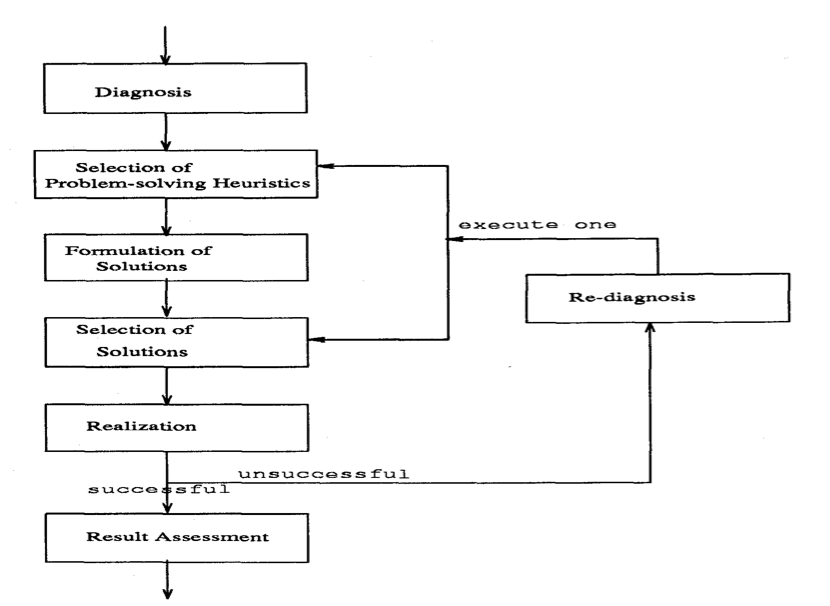
\includegraphics[height=3in]{img/ArticulationWork/mi91-awprocess.png}
	\caption[Artikulations-Prozess]{Artikulations-Prozess (entnommen aus \citep{Mi91})}
	\label{fig:img_ArticulationWork_mi91-awprocess}
\end{figure}

Die Autoren beziehen sich also offensichtlich auf explizite „Articulation Work“, die „situated“ -- beim Auftreten eines Problems im Software Engineering Prozess -- ausgelöst wird.

Zur Durchführung dieses Prozesses schlagen die Autoren einen Satz von regelbasierten Heuristiken vor, aus denen die betroffenen Individuen (hier: „agents“) auswählen können. Diese Heuristiken beschreiben mögliche Tätigkeiten im Zuge der „Articulation Work“ (ausdefiniert durch \gls{ECA}-Regelsätze). Dabei geben die Autoren Heuristiken zur Problemlösung („problem-solving heuristics“, die der direkt Behebung der aufgetretenen Probleme dienen) und Heuristiken zur Auswahl geeigneter Lösungen („selection heuristics“) an.

\subsubsection{Auswirkungen}

Das vorgeschlagene System wurde auf konzeptioneller Ebene entwickelt und nicht praktisch umgesetzt. Insofern existieren keinerlei reale Erfahrungen mit dem Ansatz. Anhand eines hypothetischen Beispiels demonstrieren die Autoren jedoch die Anwendung des Modells und der Heuristiken.

Der Vorteil liegt im Wesentlichen darin, dass der „Articulation Work“-Prozess durch seine Formalisierung bekannt ist („visible“ in Sinne der obigen Ausführungen) und dementsprechend auch offiziell auftreten „darf“. Durch den vorgegebenen Satz an Heuristiken sind außerdem die Alternativen zur Problembehandlung und deren Durchführung bekannt. Die Autoren geben diese Heuristiken für den Bereich des Software-Engineering an, betonen aber deren exemplarischen Charakter -- die Heuristiken und vor allem deren konkrete Umsetzung (durch die Spezifikation von \gls{ECA}-Regeln) müssen an die jeweilige Arbeits-Domäne angepasst werden. 

\subsubsection{Bewertung}

Das vorgeschlagene Prozess-Modell von „Articulation Work“ bildet den Ablauf auf so abstrakter Ebene ab, dass es für „situated explicit Articulation Work“ zur Lösung unmittelbar auftretender Probleme allgemein (d.h. unabhängig von der Anwendungsdomäne anwendbar erscheint.

Die Angabe von (exemplarischen) Heuristiken zur Durchführung des Artikulations-Prozesses erscheint insofern sinnvoll, als dass diese domänen- und organisations-spezifische Lösungsstrategien auch für unerfahrene Teilnehmer zugänglich machen können.

In Bezug auf die Generalisierbarkeit des Ansatzes problematisch zu sehen ist jedoch die Verwendung von \gls{ECA}-Regeln zur Spezifikation der Durchführung der einzelnen Heuristiken. Die Angabe derartiger Regeln erscheint nicht in allen Anwendungsbereichen in einem sinnvollen Detaillierungsgrad möglich zu sein. Vor allem soziale Prozesse in kooperativen Umgebungen, auf die die Autoren der ursprünglichen Literatur zum Thema „Articulation Work“ stark Bezug nehmen, können in diesen Regeln nicht sinnvoll (im Sinne einer Durchführungsvorschrift) abgebildet werden.
\\[1em]
\begin{tabular}{| p{3cm} | p{10cm} |}
  \hline
  Domäne & Software Engineering \\ \hline
  Art von AW & situated explizit \\ \hline
  Unterstützung & \emph{organisational} durch Formalisierung und a-priori-Spezifikation des Articulation-Prozesses („Was?“) und dessen Ausgestaltung („Wie?“) \\ \hline
  Auswirkungen & Definiertes Vorgehen, wie „Articulation Work“ durchgeführt werden muss \\ \hline
\end{tabular}

% subsection subsection_name (end)

\subsection{Taking CSCW seriously: Supporting Articulation Work}

\citet{Schmidt92} begründen mit dieser Arbeit eine Entwicklungsrichtung der \gls{CSCW}, die neben der Unterstützung der eigentlichen produktiven Arbeit auch auf die Unterstützung von „Articulation Work“ fokussiert. Sie beschreiben damit erstmals Anforderungen an die und Möglichkeiten der technische Unterstützung von „Articulation Work“.

\subsubsection{Kontext}

\citet{Schmidt92} widmen sich in ihren Ausführungen der kooperativen Arbeit und der Unterstützung derselben durch Computersysteme. 

\subsubsection{Unterstützung}

\subsubsection{Auswirkungen}

\subsubsection{Bewertung}
Bleibt auf Ebene der Anforderungen, trifft wenig konkrete Aussagen zur Umsetzung.
\\[1em]
\begin{tabular}{| p{3cm} | p{10cm} |}
  \hline
  Domäne & \gls{CSCW} (Workflow-Support, Shared Information Spaces, Cooperative Tools)\\ \hline
  Art von AW & planned explizit, situated explizit und implizit \\ \hline
  Unterstützung & \emph{technisch} \\ \hline
  Auswirkungen & \\ \hline
\end{tabular}


\subsection{Gegenüberstellung und Zusammenfassung} % (fold)
\label{sub:gegenüberstellung_und_zusammenfassung}

% subsection gegenüberstellung_und_zusammenfassung


% subsection modeling_articulation_work_in_software_engineering_processes (end)

\subsection{Weitere Arbeiten zur Thema Articulation Work} % (fold)
\label{sub:weitere_arbeiten_zur_thema_articulation_work}

Die im Folgenden genannten Arbeiten beziehen sich in Einzelaspekten ebenfalls auf „Articulation Work“, treffen jedoch keine Aussage hinsichtlich einer etwaigen Unterstützung derselben. Zumeist wird „Articulation Work“ als erklärendes Rahmenwerk für beobachtete Phänomene verwendet und in der Folge das Hauptaugenmerk auf diese gelegt, ohne nochmals näher auf „Articulation Work“ einzugehen. Aufgenommen wurden auch jene Arbeiten, die sich mit der grundlegenden Konzeption von Articulation Work beschäftigen (und deshalb oben bereits im Detail behandelt wurden), aber keine Aussage zur Unterstützung von „Articulation Work“ treffen. In chronologischer Reihenfolge des Erscheinens trifft dies auf folgende Arbeiten zu:
\begin{description}
	\item[\citet{Strauss85}] prägt in dieser Arbeit den Begriff „Articulation Work“ und beschreibt dieses auf konzeptioneller Ebene ohne eine unmittelbaren Praxis- bzw. Umsetzungsbezug herzustellen.
	\item[\citet{Gasser86}] beschreibt die Integration von Computerunterstützung in alltägliche Arbeitsabläufe und die Anpassungsleistung der arbeitenden Individuen, wenn die aktuelle Arbeitssituation nicht mehr mit dem der Computerunterstützung zugrunde liegenden Modell übereinstimmt. Er identifiziert dabei spezifische Aktivitäten, die im Rahmen der ablaufenden „Articulation Work“ auftreten können.
	\item[\citet{Gerson86}] zeigen die konkrete Manifestation von Articulation Work in einer Fallstudie aus einem Versicherungskonzern und identifizieren daraus die organisationalen Rahmenbedingungen, die zu jenen Problemen führen, die „Articulation Work“ notwendig machen.
	\item[\citet{Bendifallah87}] untersuchen bezugnehmend auf \citet{Gasser86} „Articulation Work“ im Kontext von IT-Support-Arbeit in Unternehmen anhand von zwei Fallstudien und identifizieren dabei zwei unterschiedliche Strategien bei der Durchführung derselben. Im Detail gehen sie jedoch nicht auf die konkret zu setzenden Maßnahmen ein.
	\item[\citet{Fujimura87}] leitet die grundlegende Unterscheidung zwischen „Production Work“ und „Articulation Work“ anhand einer Fallstudie aus dem wissenschaftlich-medizinischen Forschungsbetrieb ab. Sie bleibt dabei auf konzeptueller Ebene und beschreibt die auftretenden Phänomene, geht jedoch nicht auf unterstützende Maßnahmen ein.
	\item[\citet{Strauss88}] detailliert und erweitert seine Konzepte und setzt diese in den Kontext organisationaler Projektarbeit (in dort beschrieben Verständniss im Wesentlichen identisch mit „non-routine“ „collective activity“). Anhand einer Fallstudie aus dem Krankenhaus-Organisations-Bereich zeigt er das Auftreten in der Praxis, beschäftigt sich jedoch nicht mit möglicherweise unterstützenden Interventionen.
	\item[\citet{Schmidt90}] beschreibt ein Framework für die Analyse kooperativer Arbeit und erwähnt dabei „Articulation Work“ als ein zu berücksichtigendes Konzept. Diese Arbeit bildet die Grundlage für die im Hinblick auf die Unterstützung von „Articulation Work“ relevantere Arbeit von \citet{Schmidt92}.
\end{description}

% subsection weitere_arbeiten_zur_thema_articulation_work (end)

% section unterstützung_von_articulation_work (end)

\section{Fazit} % (fold)
\label{sec:fazit}

\textbf{hier muss eine zusammenfassende Tabelle der in der Literatur verfügbaren Information rein}

Die Zielsetzung von „Articulation Work“ formulieren die Proponenten des Ansatzes - allen voran Strauss - klar aus. Offen bleiben jedoch bei allen Autoren direkten Aussagen zum eigentlichen Gegenstand von „Articulation Work“ – also Allem was von den beteiligten Individuen zu artikulieren ist – und den notwendigen Leistungen der Individuen im Prozess der Artikulation. Aussagen zu diesen Aspekten sind aber für die Entwicklung von Ansätzen zur Unterstützung von expliziter „Articulation Work“ notwendig. 

Strauss ist sich dieser Auslassung bewusst\footnote{\emph{„[\ldots] many social scientist pay almost no attention to interior activity: ignoring it, taking it for granted, but leaving it unexamined, or giving it the kind of abstract but not very detailed analysis [\ldots]“}\citep[][S. 131]{Strauss93}}, und beschäftigt sich in späteren Arbeiten \citep{Strauss93} auch mit jenen kognitiven Vorgängen, die von ihm als „thought processes“ oder „mental activities“ bezeichnet werden und die untrennbar mit jeder Art von Tätigkeit und Interaktion verbunden sind\footnote{\emph{„These [thought processes] accompany visible action, as well as precede and follow in conditional and consequential modes“}\citep[][S. 146]{Strauss93}} und diese beeinflussen\footnote{\emph{„Even well-grooved, routine action and interaction may be accompanied by thought [\ldots] directly relevant to the work at hand. As I vacuum the house, barely noticing my movements, still I give myself commands [\ldots]“}\citep[][S. 132]{Strauss93}}. 

Im Kontext der Abstimmung von Tätigkeiten kommt den „thought processes“ der Individuen große Bedeutung zu, da sie den sichtbaren individuellen Handlungen zugrunde liegen bzw. diese beeinflussen. „Articulation Work“ wirkt sich also auf die „thought processes“ der beteiligten Individuen aus. „Thought processes“ umfassen \emph{„images, imaginations, projections of scenes, [...] flashes of insight, rehearsals of action, construction and reconstruction of scenarios, the spurting up of metaphors or comparisons, the reworking and reevaluating of past scenes and one's actions within them, and so on and on“} \citep[][S. 130]{Strauss93} - also im Wesentlichen alle kognitiven Vorgänge, die unmittelbar oder mittelbar im Zusammenhang mit den sichtbaren Arbeitsaspekten, insbesondere den Tätigkeiten zur Zielerreichung und der wahrgenommenen Arbeitsumgebung, stehen. Strauss interessiert sich allerdings ausschließlich für die dynamischen Aspekte der Interaktion zwischen Individuen, nicht aber für die Ausgangspunkte und Ergebnisse der zugrunde liegenden „thought processes“.\footnote{\emph{„I use the gerund 'ing' after 'symbol' [bei der Beschreibung von 'symbolizing', Anm.] to signify that my principal interest is, again, in interaction rather than its products, for symbols are precipitates of interaction“}\citep[][S. 149]{Strauss93}}  Wie bereits oben erwähnt sind aber die Repräsentationen, auf den „thought processes“ beruhen und operieren, für die Unterstützung von „Articulation Work“ von Interesse. Die kognitions-wissenschaftlichen Ansätze zu Schemata (\citep{Rumelhart78} \citep[vgl. nach ][]{Hanke06}) und mentalen Modellen (\citep[vgl. ][]{Seel91}) sind ein Erklärungsansatz für diese Lücke.

% section fazit (end)
% chapter articulation_work (end)

